%% Ch.04-20   | Spark Operations
%
\subsection{Spark Operations}\label{subsec:spark-operations}
\begin{frame}
    \frametitle{Spark Operations}
    \begin{itemize}
        \item Spark \textbf{operations} on distributed data can be classified into two types: transformations
        and actions.
        \item All spark operations are \texttt{\color{blue}{immutable}}.
    \end{itemize}
\end{frame}
\begin{frame}
    \frametitle{Immutable Objects}
    \begin{itemize}
        \item An object whose state cannot change after it has been constructed is
        called immutable (unchangable).\footnote{Referenced from https://otfried.org/courses/cs109scala/tutorial_mutable.html}
        \item  The methods of an immutable object do not modify the state of the object.
    \end{itemize}
\end{frame}

\begin{frame}
    \frametitle{Immutable Objects}
    \begin{figure}
        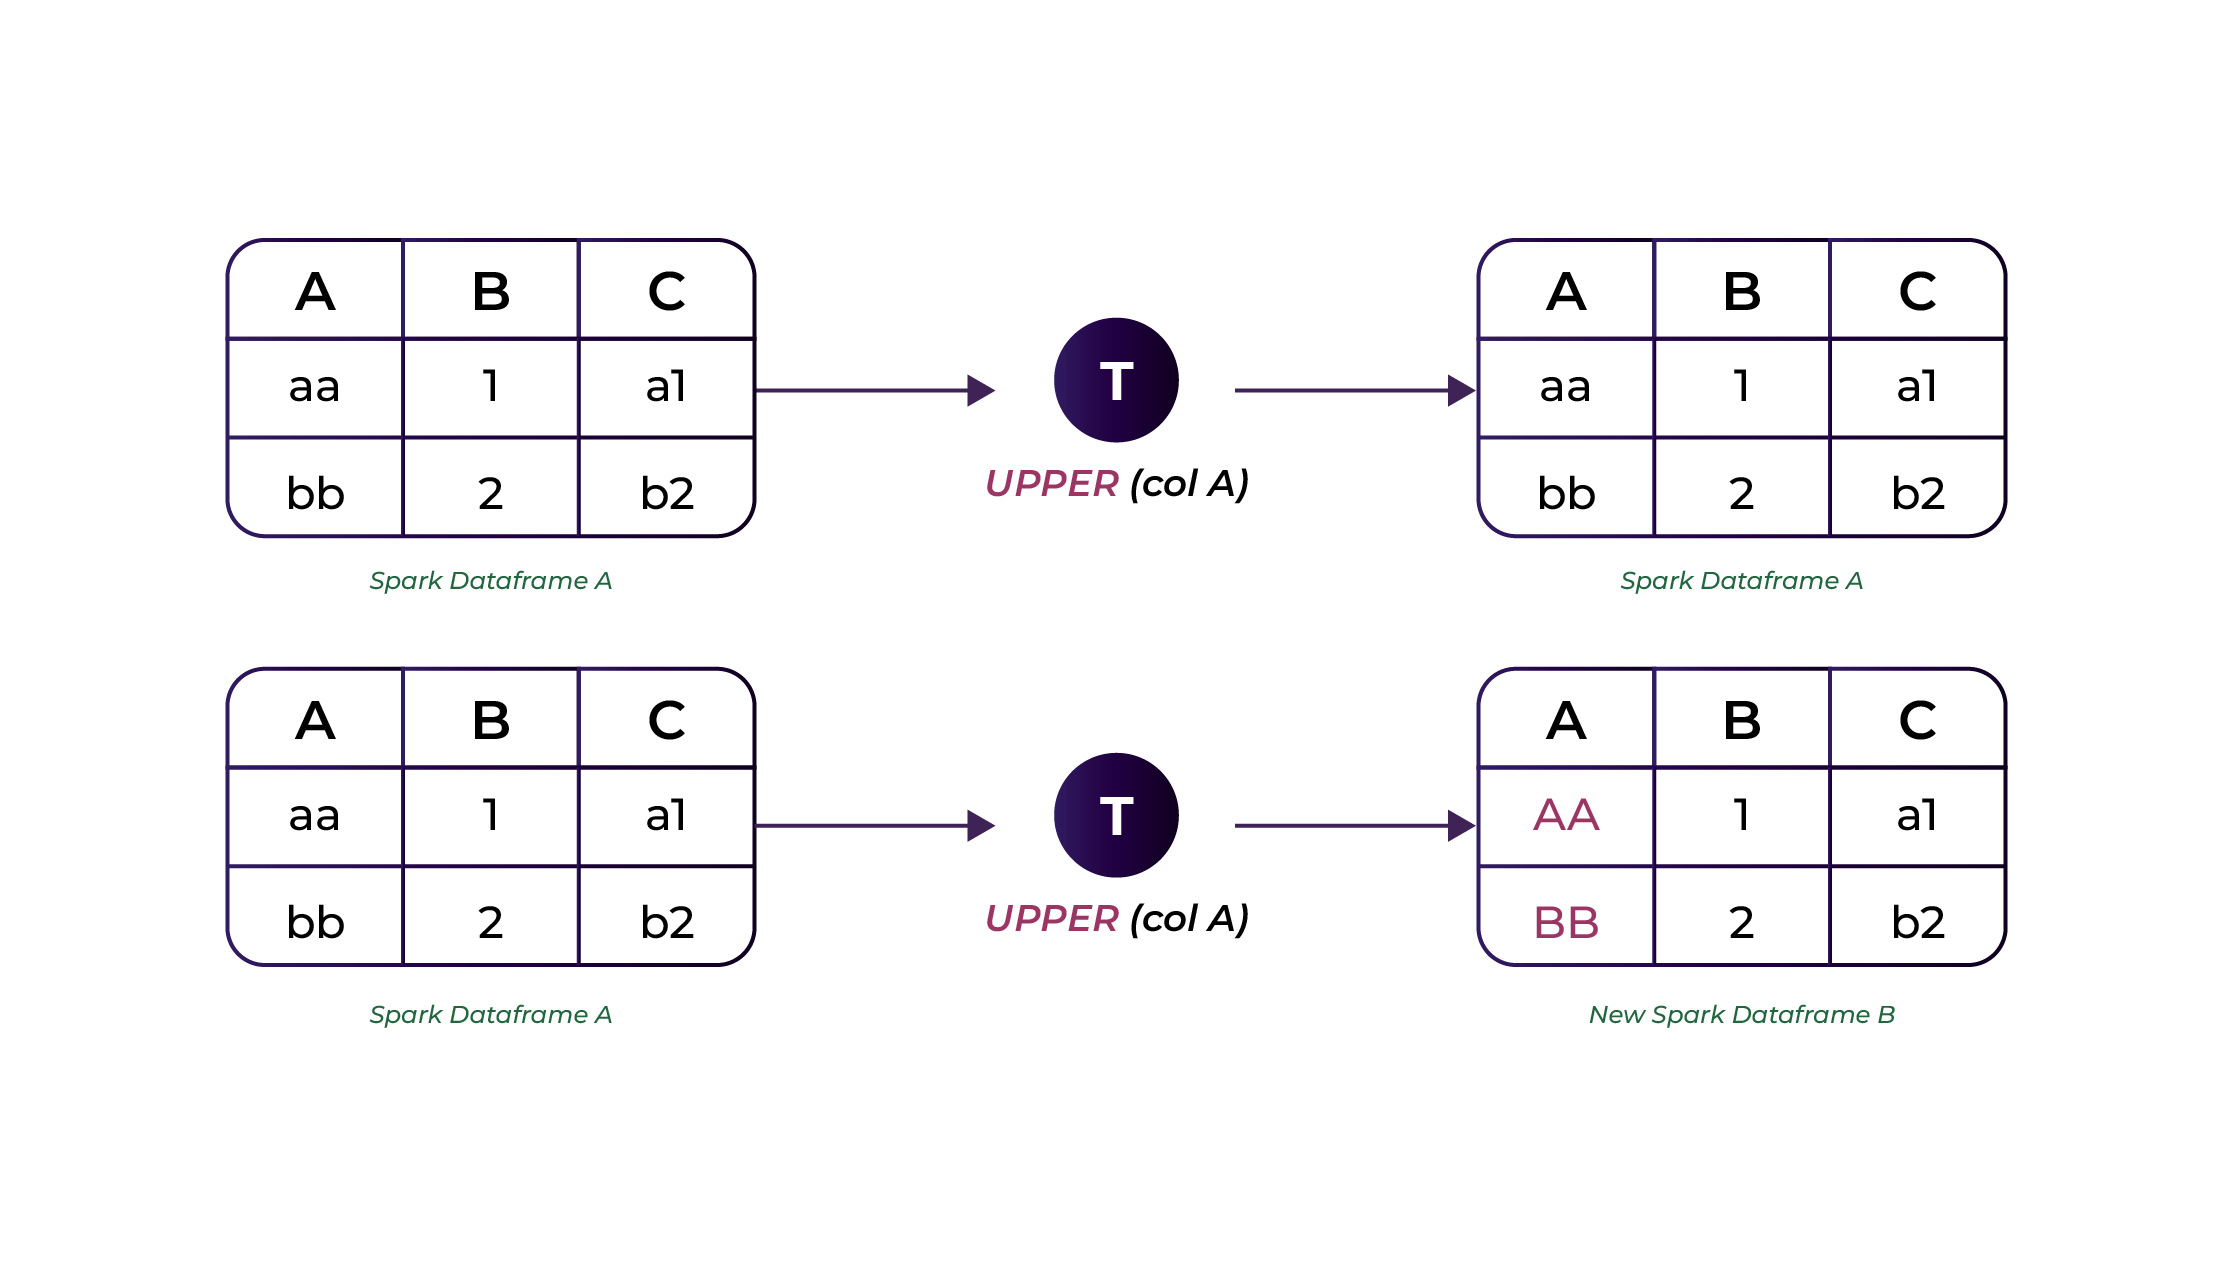
\includegraphics[width=\textwidth,height=.7\textheight,keepaspectratio]{./Figures/chapter-04/Immutable_df}
        \caption{Spark Dataframe is immutable, and you can't change its values.}\label{fig:Immutable_df}
    \end{figure}
\end{frame}

\begin{frame}[fragile]
    \frametitle{Immutable Objects}
    \begin{figure}
        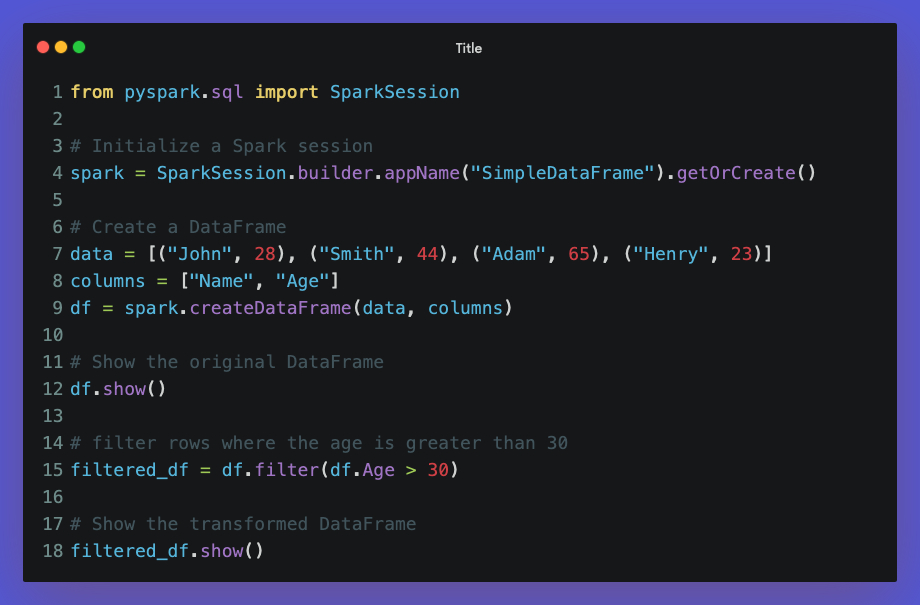
\includegraphics[width=\textwidth,height=.75\textheight,keepaspectratio]{./Figures/chapter-04/pyspark_immutable_df}
        \caption{Filtering a PySpark DataFrame Based on Age}\label{fig:pyspark_immutable_df}
    \end{figure}
\end{frame}
\begin{frame}[fragile]
    \frametitle{DEMO}
    DEMO
\end{frame}
\begin{frame}
    \frametitle{Spark Operations: Transformations}
    \begin{itemize}
        \item Transformations: transform a Spark DataFrame into a new DataFrame \textit{\color{blue}{without altering the original data}}.
        \item Example of Spark transformations, \texttt{\color{orange}{map(), select(), filter(), or drop()} }
    \end{itemize}
\end{frame}

\begin{frame}
    \frametitle{Spark Transformations: What are Lazy Transformations?}
    \begin{itemize}
        \item In Spark, transformations are \textit{lazy}.
        \item This means computations are not executed immediately.
        \item Spark builds a \textbf{DAG} (Directed Acyclic Graph) of transformations.
        \item All Transformations results are not computed immediately, but they are recorded or remembered as a \textbf{lineage}.
    \end{itemize}
\end{frame}

\begin{frame}
    \frametitle{Spark Transformations: Benefits of Lazy Evaluation}
    \begin{itemize}
        \item \textbf{Optimization:} A lineage allows Spark, at a later time in its execution plan, to rearrange certain transformations, coalesce
        them, or optimize transformations into stages for more efficient execution.
        \item \textbf{Resource Management:} Executes tasks efficiently, using fewer resources.
        \item \textbf{Fault Tolerance:} Easier to recompute parts of the pipeline if a part fails.
    \end{itemize}
\end{frame}

\begin{frame}
    \frametitle{Spark Transformations: Lazy Transformation}
    \begin{itemize}
        \item Consider a dataset with map and filter transformations.
        \item Spark does not execute these transformations when they are defined.
        \item Transformations are executed when an action (like \textbf{collect}, \textbf{count}) is called.
    \end{itemize}
\end{frame}
\begin{frame}
    \frametitle{Lazy Transformations Example}
    \begin{figure}
        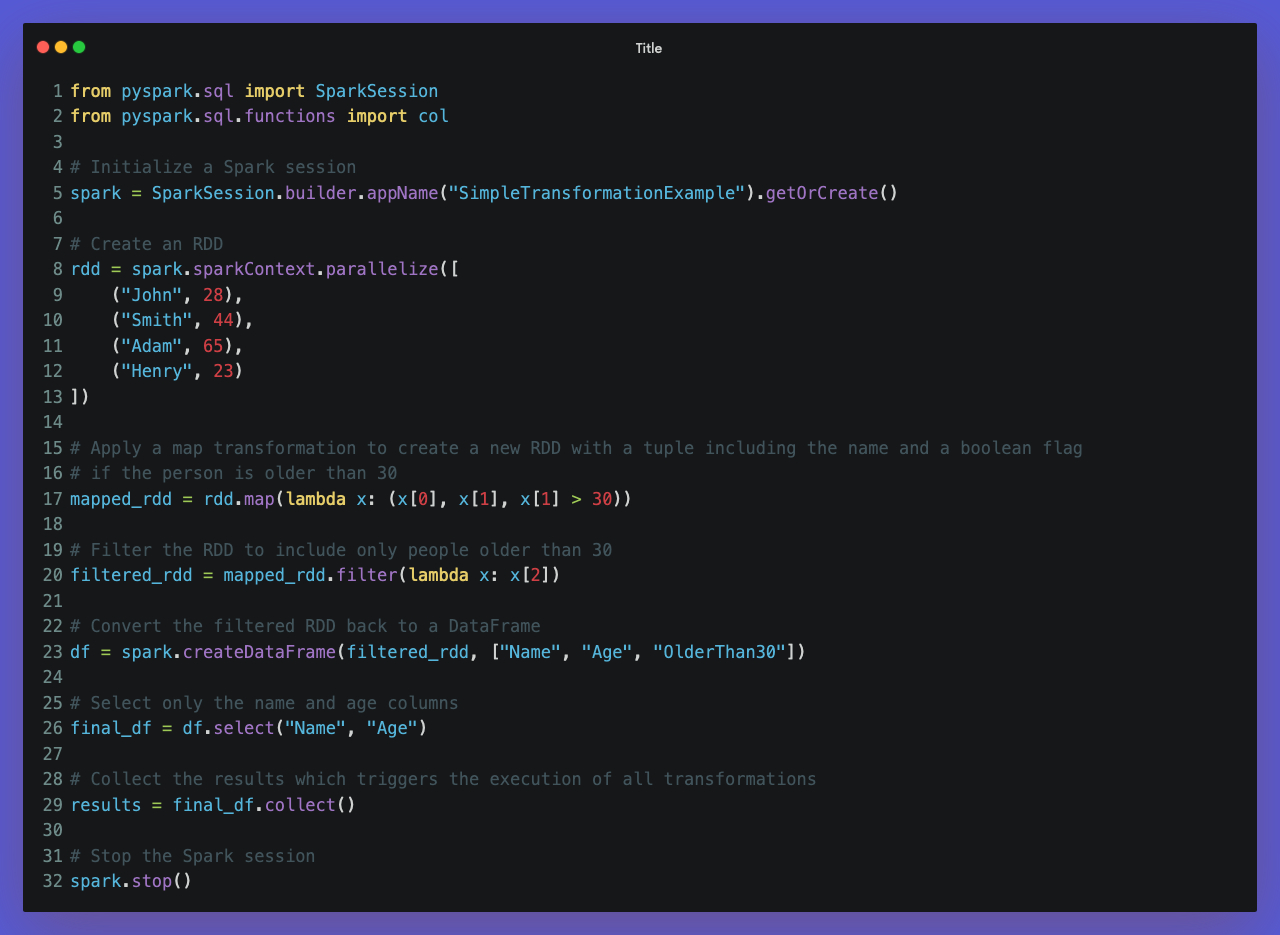
\includegraphics[width=\textwidth,height=.75\textheight,keepaspectratio]{./Figures/chapter-04/pyspark_transformations}
        \caption{Spark Lazy Transformations Example.}\label{fig:pyspark_transformations}
    \end{figure}
\end{frame}
\begin{frame}
    \frametitle{Spark Operations: Actions}
    \begin{itemize}
        \item An action triggers the lazy evaluation of all the recorded transformations.
        \item Actions are operations that trigger execution of transformations.
        \item They are used to either compute a result to be returned to the Spark driver program or to write data to an external storage system.
        \item Actions include operations like \textbf{count}, \textbf{collect}, \textbf{saveAsTextFile}, and \textbf{take}.
    \end{itemize}
\end{frame}

\begin{frame}
    \frametitle{Examples of Spark Actions}
    \begin{itemize}
        \item \textbf{collect()}: Collects all elements from the Spark context to the driver program.
        \item \textbf{count()}: Returns the number of elements in the dataset.
        \item \textbf{saveAsTextFile(path)}: Saves the dataset to a text file at the specified path.
        \item \textbf{take(n)}: Returns an array with the first n elements of the dataset.
    \end{itemize}
\end{frame}

% Ch.04-21   | Transformations Narrow Vs Wide

\subsection{Narrow and Wide Transformations}\label{subsec:narrow-and-wide-transformations}
\begin{frame}
    \frametitle{Introduction to Spark Transformations}
    \begin{itemize}
        \item Transformations create new RDDs from existing ones.
        \item Spark has two types of transformations: Narrow and Wide.
    \end{itemize}
\end{frame}

\begin{frame}
    \frametitle{What are Narrow Transformations?}
    \begin{itemize}
        \item Transformations that do not require data shuffling between partitions.
        \item Examples: \texttt{map()}, \texttt{filter()}.
        \item Data processing is limited to a single partition.
    \end{itemize}
\end{frame}

\begin{frame}
    \frametitle{What are Narrow Transformations?}
    \begin{figure}
        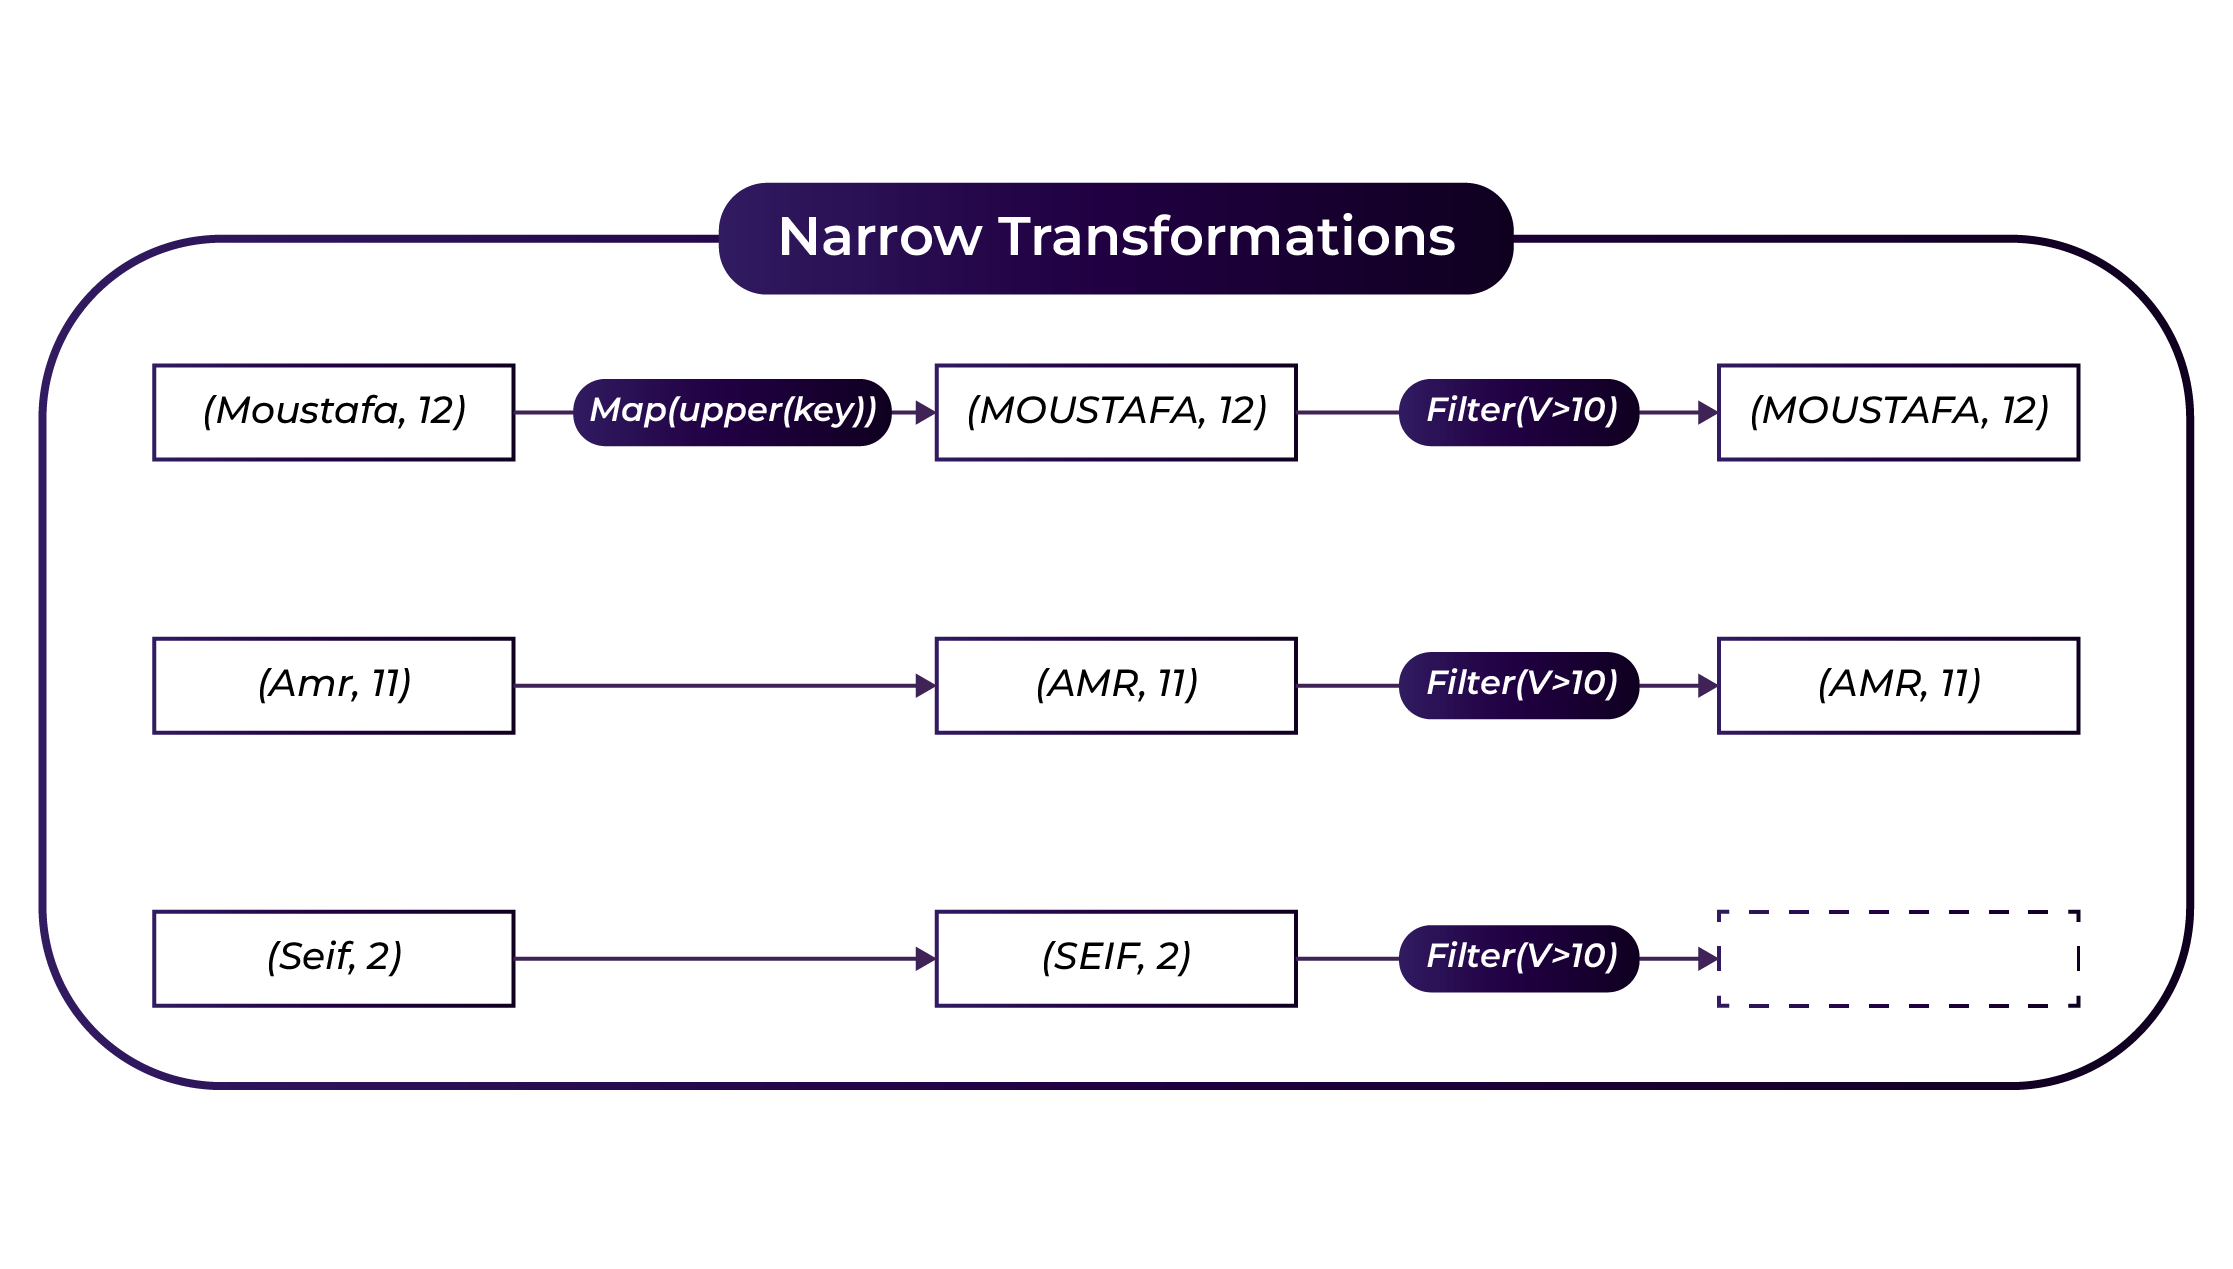
\includegraphics[width=\textwidth,height=.75\textheight,keepaspectratio]{./Figures/chapter-04/Narrow}
        \caption{Spark Narrow Transformations.}\label{fig:spark_narrow}
    \end{figure}
\end{frame}

\begin{frame}
    \frametitle{Benefits of Narrow Transformations}
    \begin{itemize}
        \item Efficient with minimal data movement.
        \item Best for independent data processing tasks.
    \end{itemize}
\end{frame}

\begin{frame}
    \frametitle{What are Wide Transformations?}
    \begin{itemize}
        \item Transformations that involve shuffling data across partitions.
        \item Examples: \texttt{groupBy()}, \texttt{reduceByKey()}.
    \end{itemize}
\end{frame}

\begin{frame}
    \frametitle{What are Wide Transformations?}
    \begin{figure}
        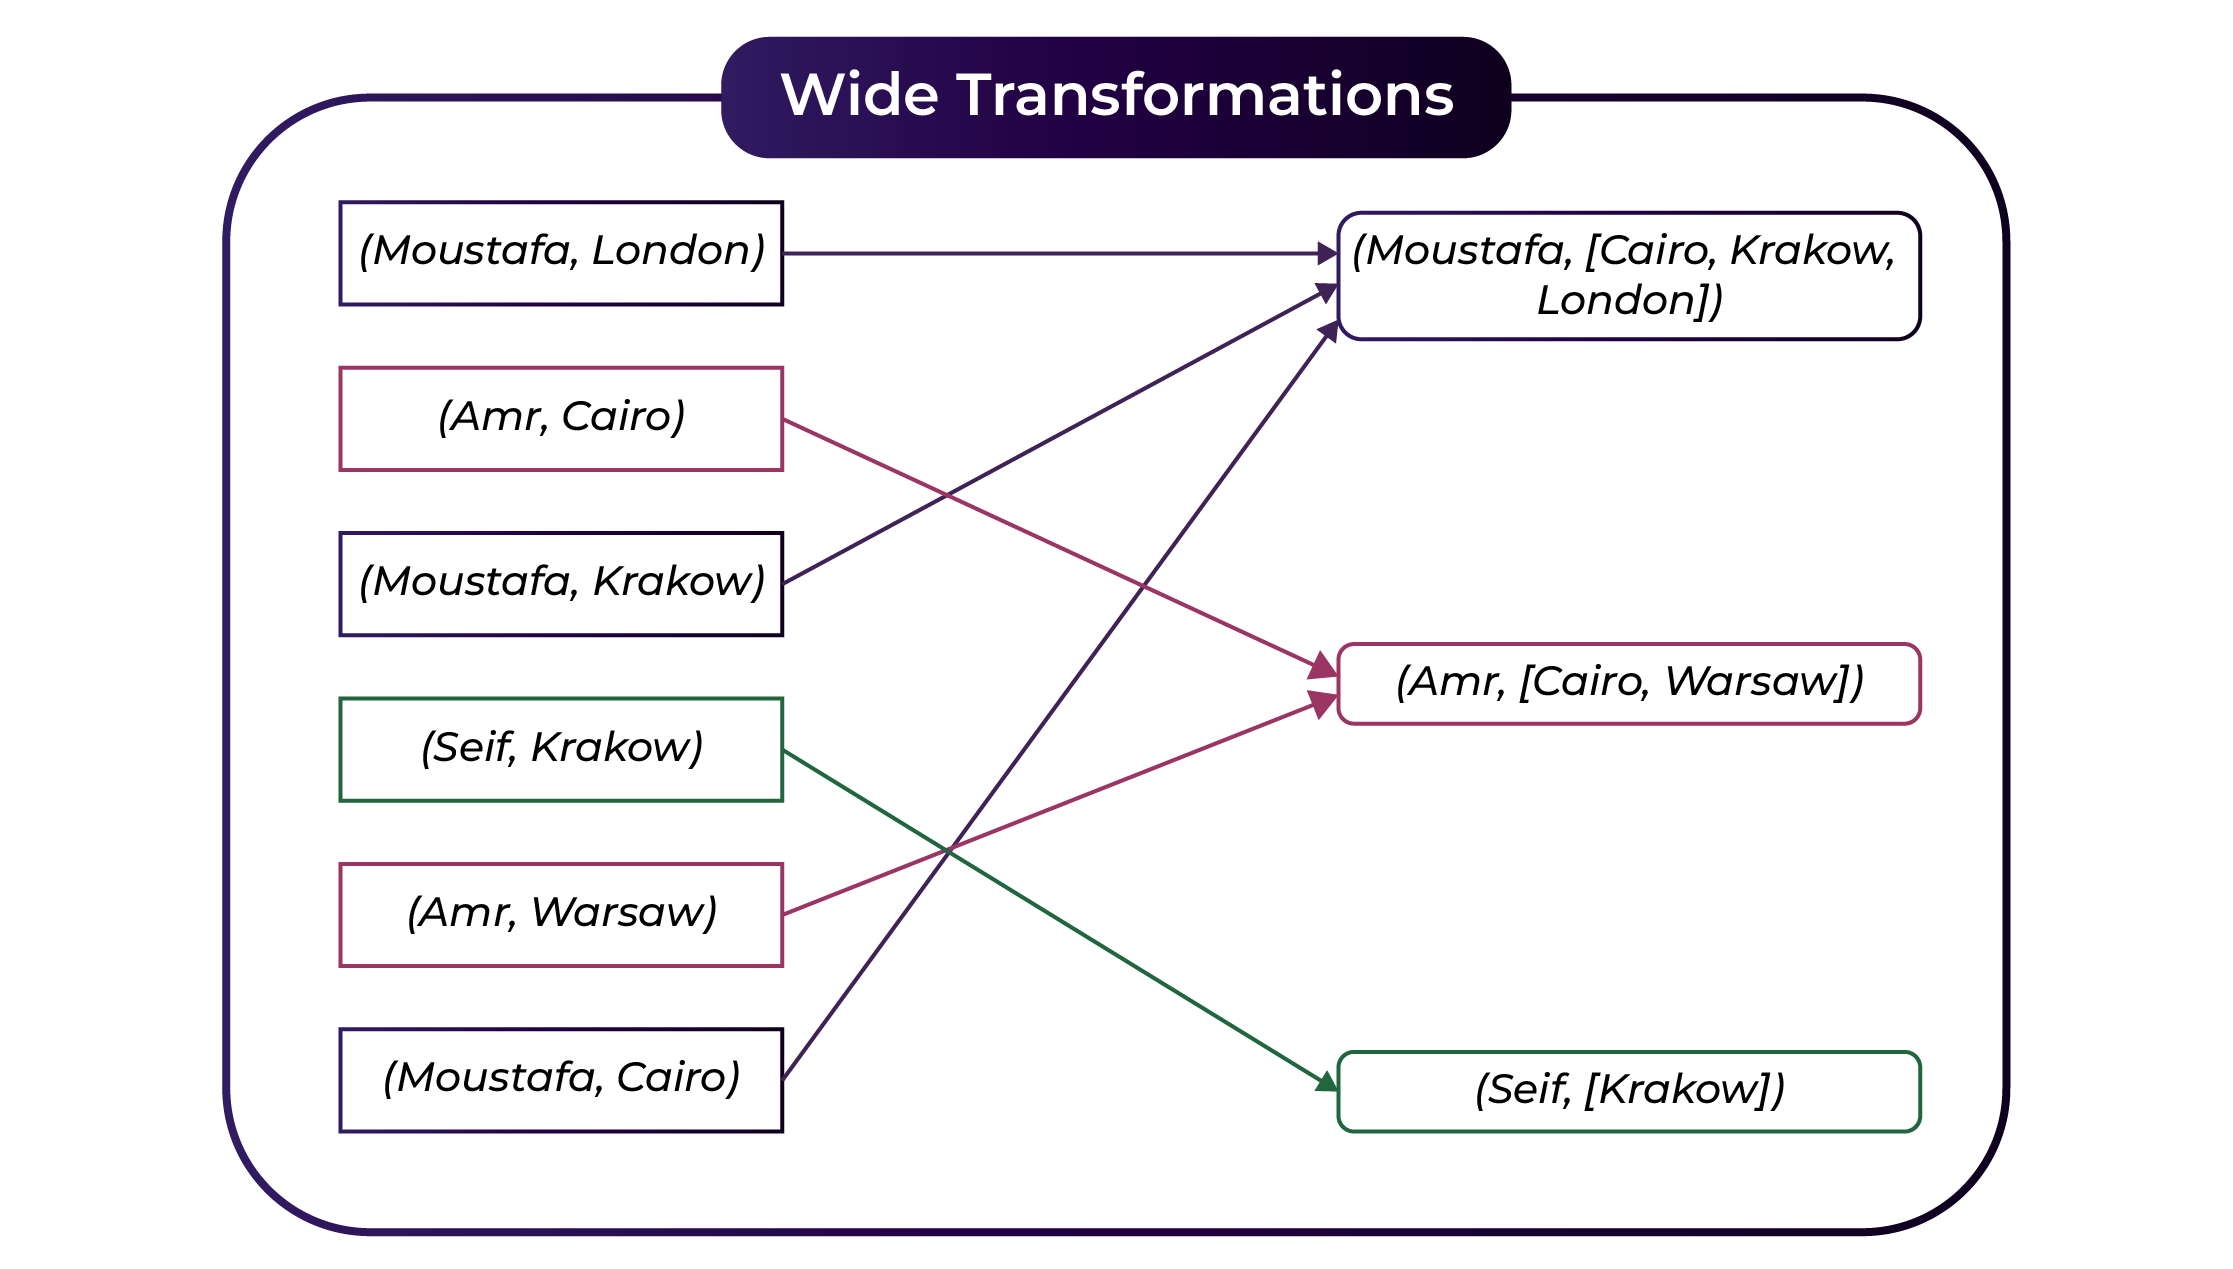
\includegraphics[width=\textwidth,height=.75\textheight,keepaspectratio]{./Figures/chapter-04/Wide}
        \caption{Spark Wide Transformations.}\label{fig:spark_wide}
    \end{figure}
\end{frame}

\begin{frame}
    \frametitle{Wide Transformations and Dependencies}
    \begin{itemize}
        \item \textbf{Wide Dependencies}: Require data from multiple partitions, often involving shuffling.
        \item \textbf{Examples}: \texttt{groupBy()}, \texttt{orderBy()} - data is combined across partitions, affecting performance.
        \item \textbf{Impact}: These transformations are necessary for operations like counting occurrences across a dataset.
    \end{itemize}
\end{frame}

\begin{frame}
    \frametitle{Implications of Wide Transformations}
    \begin{itemize}
        \item Shuffling can be expensive in terms of time and network I/O.
        \item Essential for aggregation and grouping operations.
    \end{itemize}
\end{frame}

\begin{frame}
    \frametitle{Narrow vs. Wide Dependencies}
    \begin{itemize}
        \item \textbf{Narrow Dependencies}: A single output partition can be computed from a single input partition without data exchange.
        \item \textbf{Examples}: \texttt{filter()}, \texttt{contains()} - operate independently on partitions.
    \end{itemize}
\end{frame}

\subsection{Repartition vs. Coalesce}\label{subsec:repartition-vs-coalesce}
\begin{frame}
    \frametitle{Repartition vs. Coalesce}
    \begin{itemize}
        \item In Apache Spark, repartition and coalesce are two methods used to change the number of partitions in an RDD (Resilient
        Distributed Dataset).
    \end{itemize}
\end{frame}

\begin{frame}
    \frametitle{Repartition vs. Coalesce}

    \begin{table}[h!]
        \centering
        \resizebox{\textwidth}{!}{%
            \begin{tabular}{|p{2cm} |p{6cm} |p{6cm} |}
                \hline
                \rowcolor{Gray}
                \hline
                \textbf{Aspect}    & \textbf{Repartition}  & \textbf{Coalesce} \\
                \hline
                \textbf{Purpose}   & \textcolor{blue}{Increases or decreases} the number of partitions. & \textcolor{blue}{Decreases} the number of partitions. \\
                \hline
                \textbf{Mechanism} & \textcolor{blue}{Shuffles all} the data across the network to create a new set of partitions. & \textcolor{blue}{Merges existing} partitions \textcolor{blue}{without} a full data shuffle. \\
                \hline
                \textbf{Use Case}  & Ideal for increasing the number of partitions or significantly \textcolor{blue}{changing the distribution} of data. & Efficient for \textcolor{blue}{reducing the number} of partitions when the target number is less than the current number. \\
                \hline
                \textbf{Cost}      & Expensive due to the \textcolor{blue}{full data shuffle}. & Less expensive than \texttt{repartition} as it \textcolor{blue}{minimizes data movement}. \\
                \hline
            \end{tabular}
        }
        \caption{Comparison of Repartition and Coalesce in Apache Spark}\label{tab:rerepartition-coalesce}
    \end{table}
\end{frame}

%\begin{frame}[fragile]
%    \frametitle{High-Level Code: Repartition}
%    \begin{lstlisting}[language=scala,label={lst:rep-partition},caption={Repartition Code}]
%def repartition(numPartitions: Int)(implicit ord: Ordering[T] = null): RDD[T] = withScope {
%  coalesce(numPartitions, shuffle = true)
%}
%    \end{lstlisting}
%    \begin{itemize}
%        \item \textbf{Key Points}:
%        \begin{itemize}
%            \item \textbf{Shuffle}: Always performs a shuffle by calling `coalesce` with `shuffle = true`.
%            \item \textbf{Usage}: Suitable for both increasing and decreasing the number of partitions with even data distribution.
%        \end{itemize}
%    \end{itemize}
%\end{frame}
%
%\begin{frame}
%    \frametitle{High-Level Code: Repartition}
%
%        \begin{itemize}
%            \item \textbf{Operation}: Calls `coalesce` with `shuffle = true`.
%            \item \textbf{Process}: Full data shuffle across the network to redistribute data evenly.
%            \item \textbf{Impact on Logs}:
%            \begin{itemize}
%                \item Increased log entries due to extensive shuffle operations.
%                \item Higher overhead and cost.
%                \item Useful for balancing load and increasing parallelism.
%            \end{itemize}
%        \end{itemize}
%\end{frame}
%
%\begin{frame}
%    \frametitle{High-Level Code: Repartition}
%    \begin{itemize}
%        \item Shuffling Logic (If shuffle is true):
%
%            \begin{itemize}
%                \item Data is shuffled to distribute it evenly across the new partitions.
%                \item Each item is assigned a new partition based on a random function.
%                \item A new RDD is created with the shuffled data and the specified number of partitions.
%            \end{itemize}
%        \end{itemize}
%\end{frame}
%
%\begin{frame}[fragile]
%    \frametitle{High-Level Code: Coalesce}
%
%    \begin{lstlisting}[language=scala,basicstyle=\tiny,label={lst:coalesce},caption={Coalesce Code}]
%def coalesce(numPartitions: Int, shuffle: Boolean = false,
%             partitionCoalescer: Option[PartitionCoalescer] = Option.empty)
%            (implicit ord: Ordering[T] = null): RDD[T] = withScope {
%  require(numPartitions > 0, s"Number of partitions ($numPartitions) must be positive.")
%  if (shuffle) {
%    // Shuffle logic
%    val distributePartition = (index: Int, items: Iterator[T]) => {
%      var position = new XORShiftRandom(index).nextInt(numPartitions)
%      items.map { t =>
%        position = position + 1
%        (position, t)
%      }
%    } : Iterator[(Int, T)]
%    new CoalescedRDD(new ShuffledRDD[Int, T, T](
%        mapPartitionsWithIndexInternal(distributePartition, isOrderSensitive = true),
%        new HashPartitioner(numPartitions)),
%      numPartitions,
%      partitionCoalescer).values
%  } else {
%    // No-shuffle logic
%    new CoalescedRDD(this, numPartitions, partitionCoalescer)
%  }
%}
%    \end{lstlisting}
%
%\end{frame}
%
%\begin{frame}[fragile]
%    \frametitle{High-Level Code: Coalesce}
%    \begin{itemize}
%        \item \textbf{Key Points}:
%        \begin{itemize}
%            \item \textbf{Shuffle}: Optional; can perform a shuffle if `shuffle = true`.
%            \item \textbf{No Shuffle}: Default behavior (without shuffle) merges partitions locally.
%            \item \textbf{Usage}: Efficient for reducing the number of partitions without shuffling.
%        \end{itemize}
%    \end{itemize}
%\end{frame}
%
%
%
%
%\begin{frame}
%    \frametitle{High-Level Code: Coalesce}
%
%    \begin{itemize}
%        \begin{itemize}
%            \item \textbf{Operation}: Can operate with or without shuffle.
%            \item \textbf{Process}:
%            \begin{itemize}
%                \item \textbf{No Shuffle (default)}: Merges partitions locally.
%                \item \textbf{With Shuffle}: Performs a shuffle for even data distribution if specified.
%            \end{itemize}
%            \item \textbf{Impact on Logs}:
%            \begin{itemize}
%                \item Decreased log entries when merging locally without shuffle.
%                \item Lower overhead and cost.
%                \item Efficient for reducing partitions, especially useful for write operations.
%                \item Optional shuffle provides flexibility for balanced distribution.
%            \end{itemize}
%        \end{itemize}
%    \end{itemize}
%\end{frame}
%
%\subsection{Understanding Spark Application Concepts}\label{subsec:understanding-spark-application-concepts}
%
%\begin{frame}
%    \frametitle{Understanding Spark Application Concepts}
%    \begin{itemize}
%        \item \textbf{Job}: A parallel computation consisting of multiple tasks that gets spawned in response
%        to a Spark action (e.g., save(), collect()).
%        \item \textbf{Stage}: Each job gets divided into smaller sets of tasks called stages that depend on each
%        other.
%        \item \textbf{Task}: A single unit of work or execution that will be sent to a Spark executor.
%    \end{itemize}
%\end{frame}
%
%\begin{frame}
%    \frametitle{Spark Jobs}
%    \begin{figure}
%        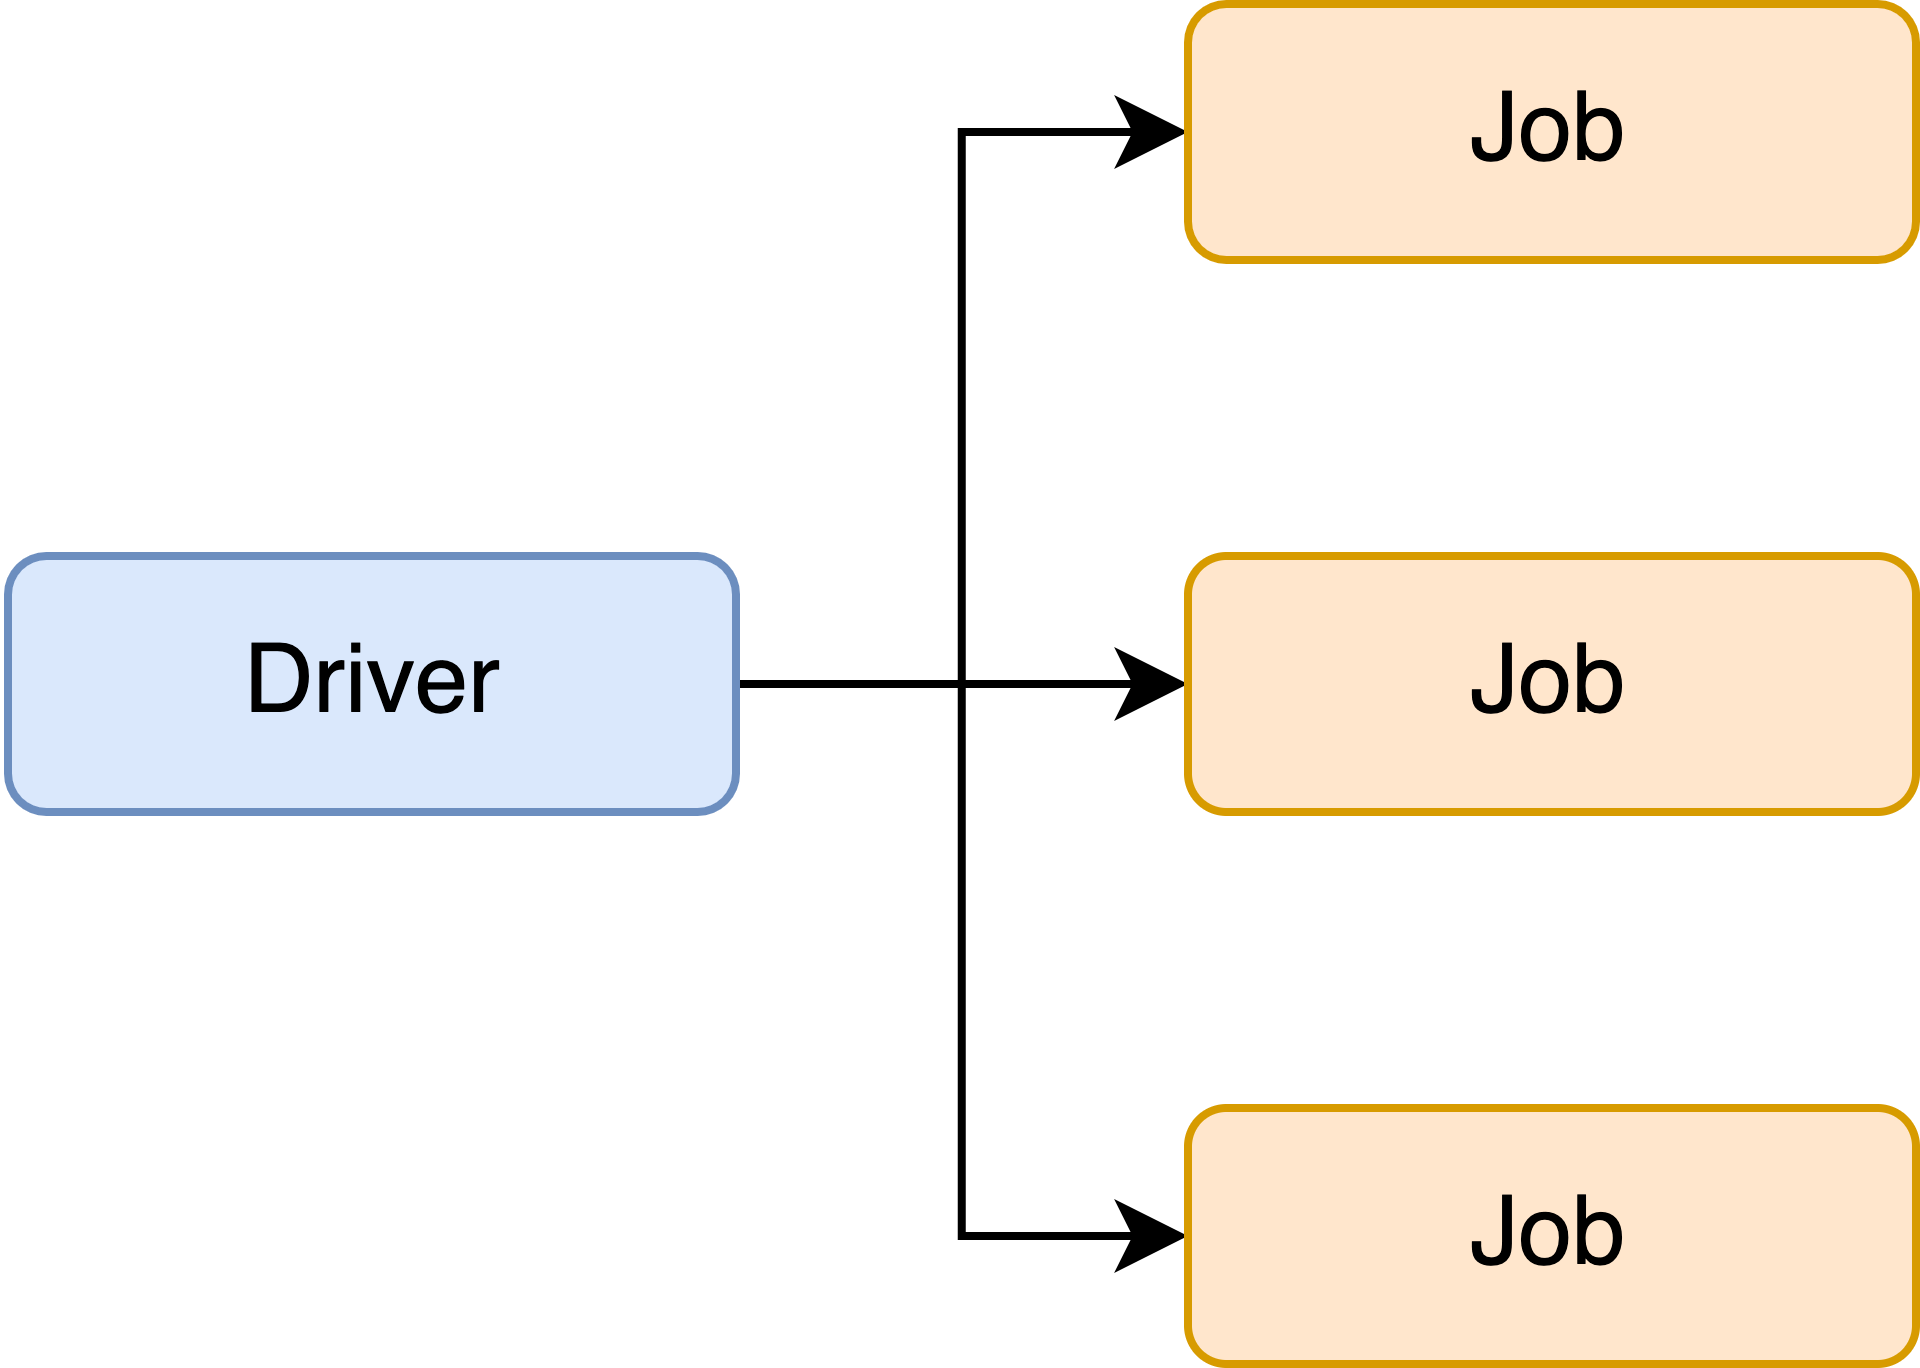
\includegraphics[width=\textwidth,height=.7\textheight,keepaspectratio]{./Figures/chapter-04/spark_job}
%        \caption{Spark driver creating one or more Spark jobs.}\label{fig:spark_job}
%    \end{figure}
%\end{frame}
%
%\begin{frame}
%    \frametitle{Spark Stages}
%    \begin{figure}
%        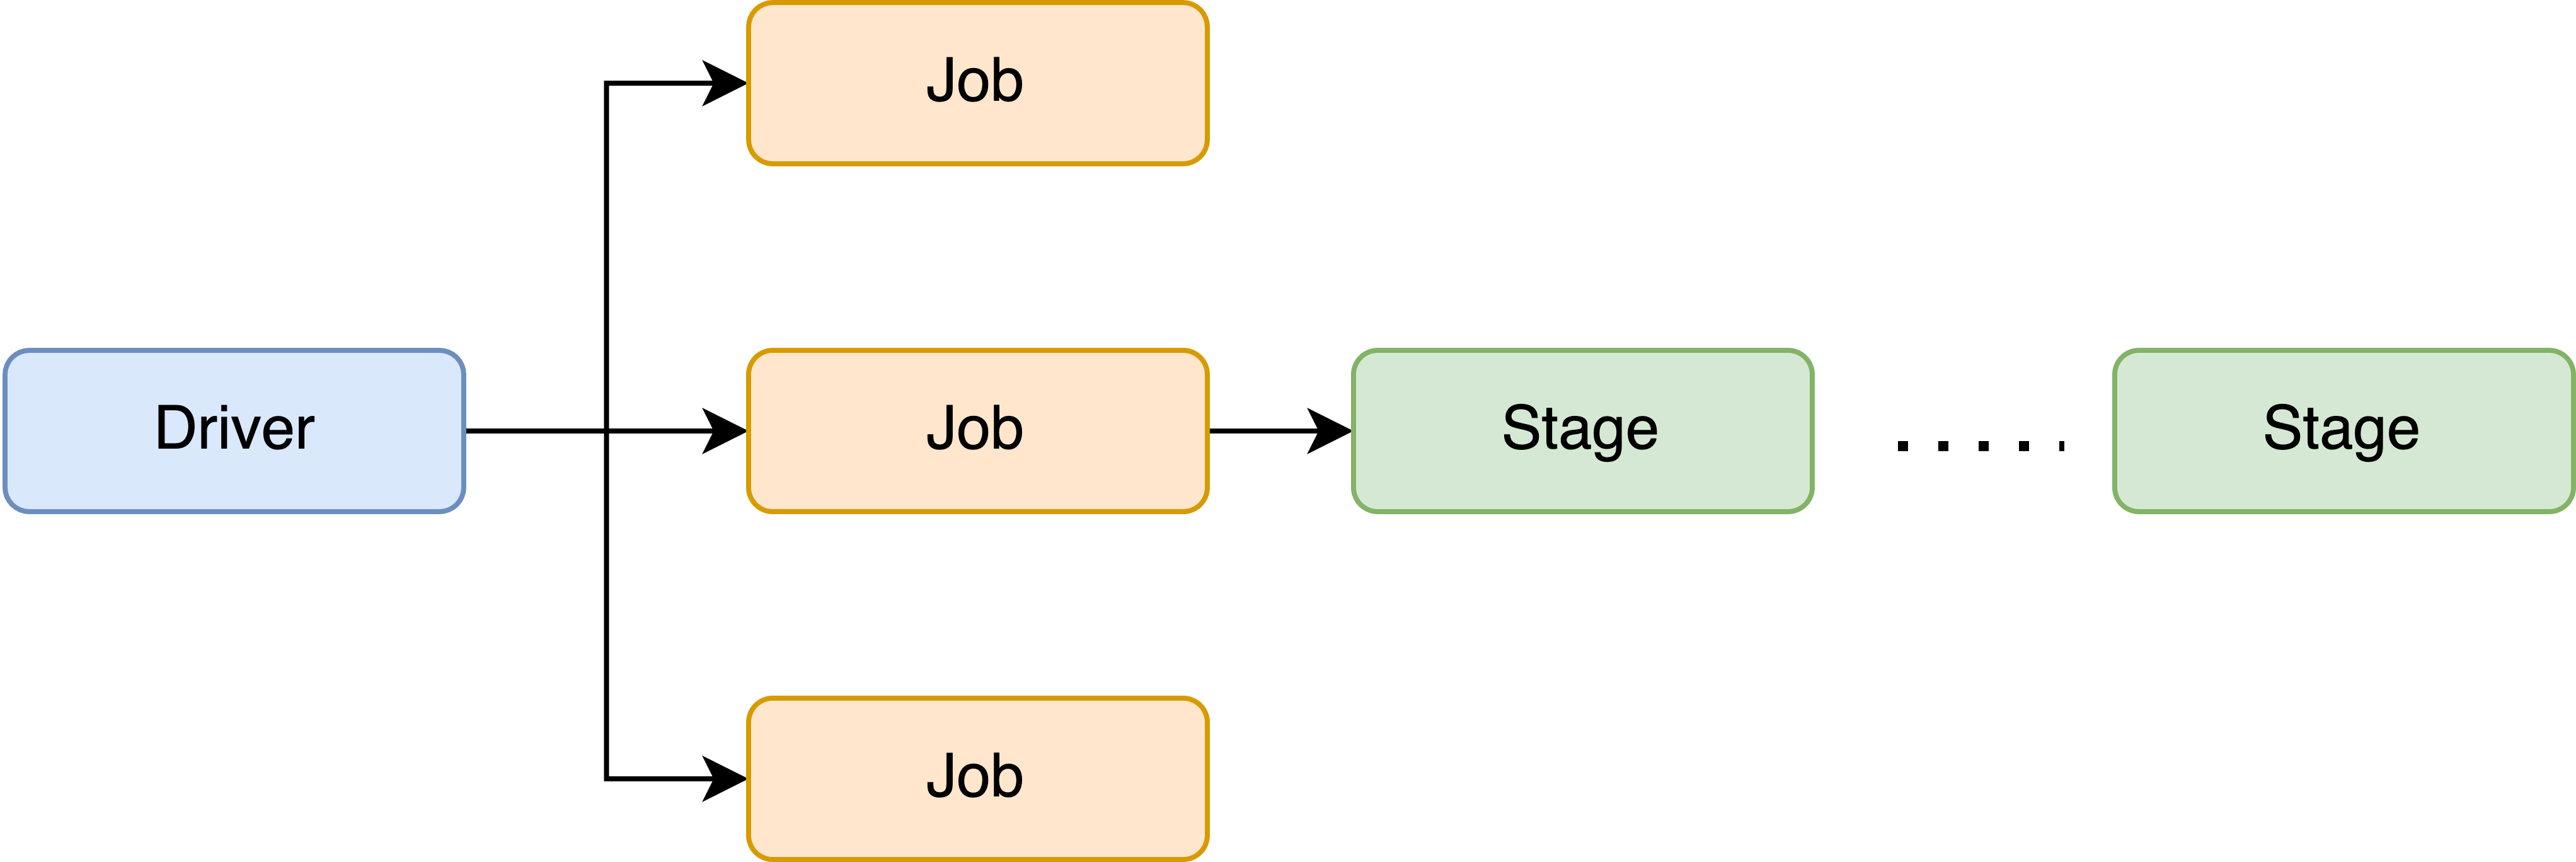
\includegraphics[width=\textwidth,height=.65\textheight,keepaspectratio]{./Figures/chapter-04/Spark_Stages}
%        \caption{Spark job creating one or more stages}\label{fig:spark_stages}
%    \end{figure}
%\end{frame}
%
%\begin{frame}
%    \frametitle{Spark Stages}
%    \begin{figure}
%        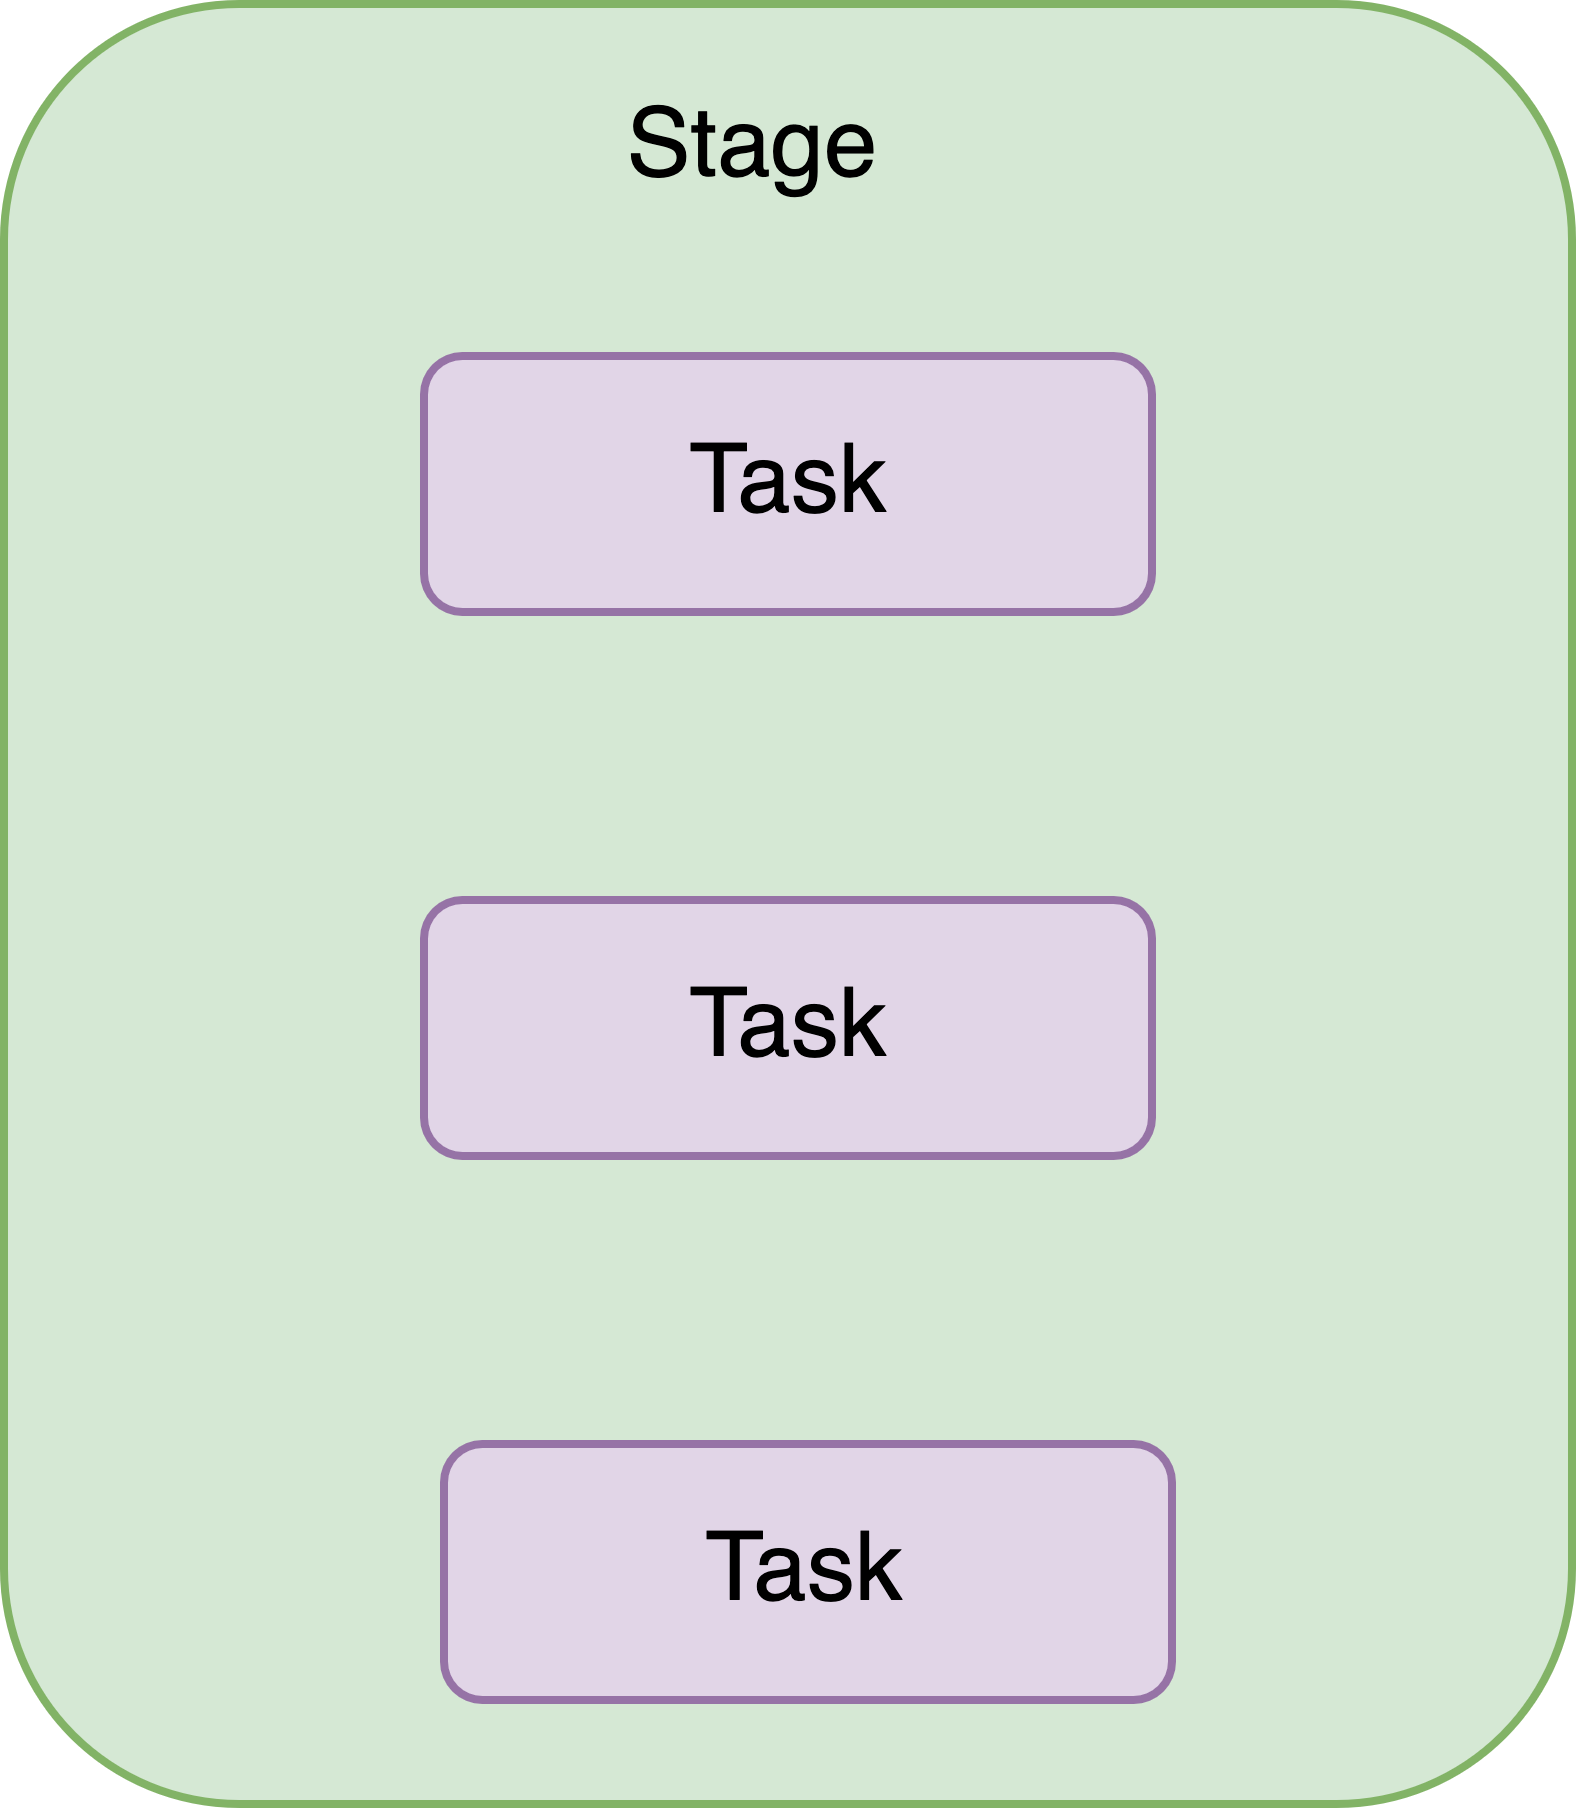
\includegraphics[width=\textwidth,height=.7\textheight,keepaspectratio]{./Figures/chapter-04/Spark_Stage}
%        \caption{Spark stage creating one or more tasks to be distributed to executors}\label{fig:spark_stage}
%    \end{figure}
%\end{frame}

%\begin{frame}
%    \frametitle{Spark Tasks}
%    \begin{figure}
%        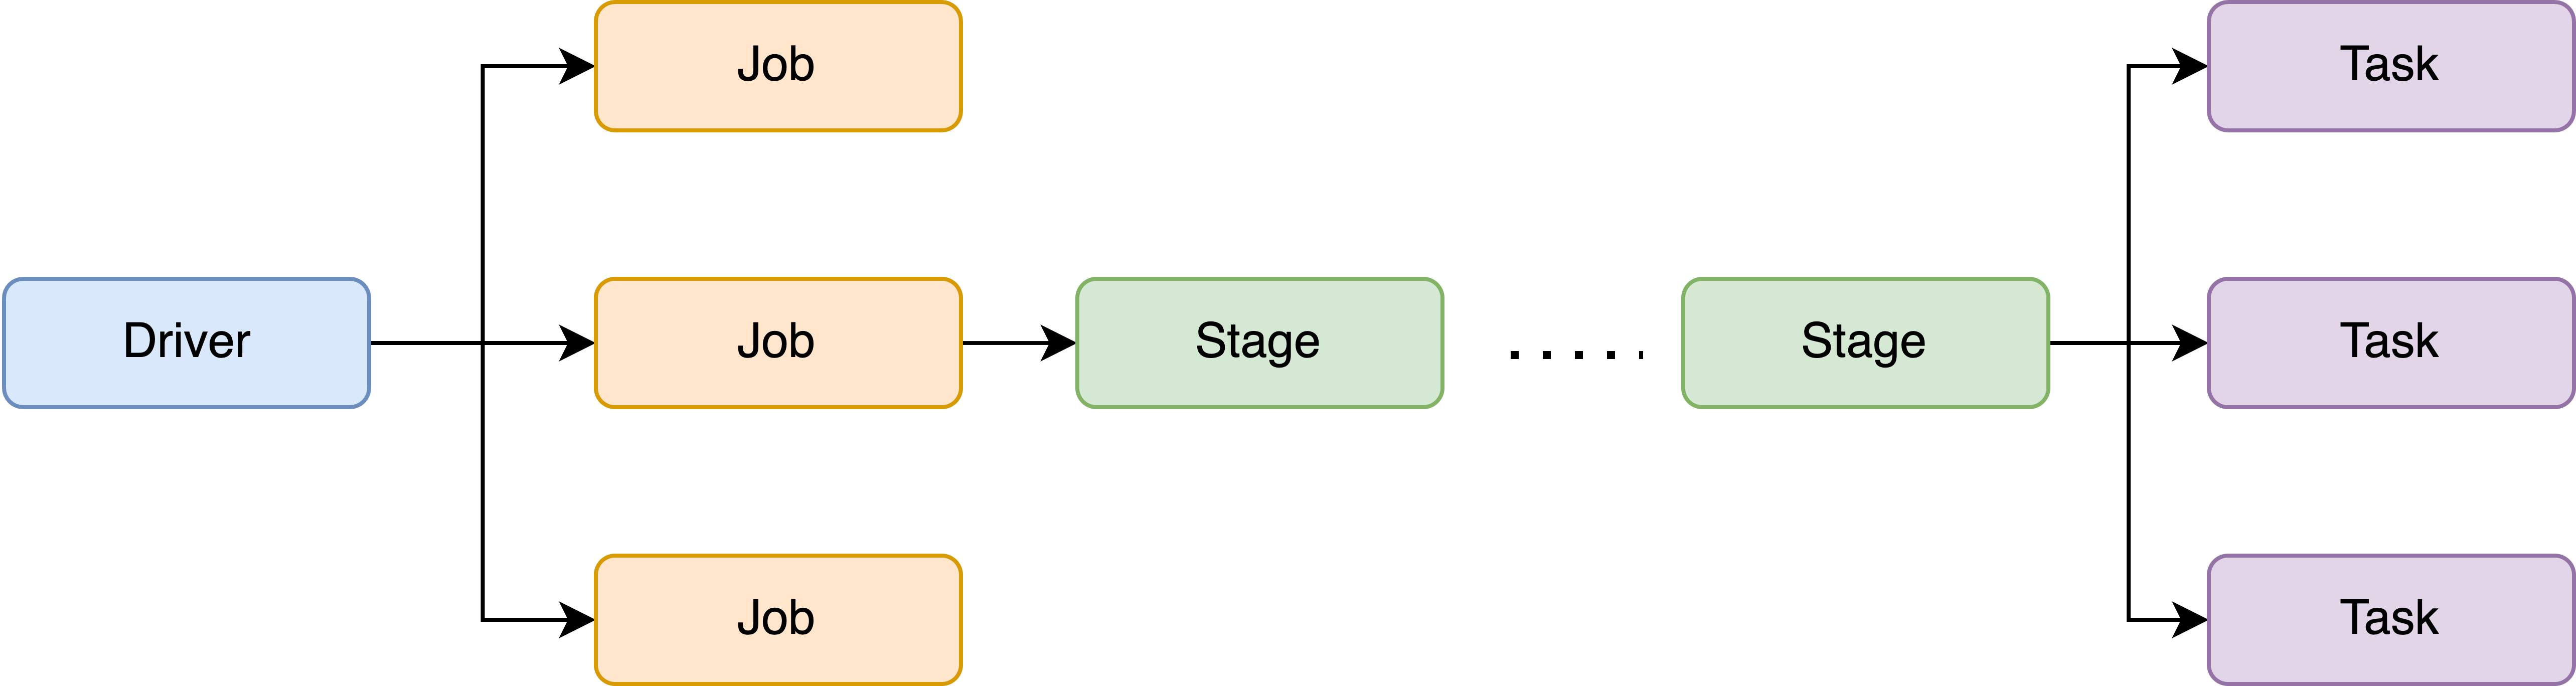
\includegraphics[width=\textwidth,height=.7\textheight,keepaspectratio]{./Figures/chapter-04/Spark_tasks}
%        \caption{Spark stage creating one or more tasks to be distributed to executors}\label{fig:Spark_tasks}
%    \end{figure}
%\end{frame}
%
%\subsection{Running Word Count \& Aggregation using Spark}\label{subsec:running-word-count-&-aggregation-using-spark}
%
%\subsection{Spark Application Life Cycle}\label{subsec:spark-application-life-cycle}
%%%%% Later
%\begin{frame}
%    \frametitle{The Life Cycle of a Spark Application (Inside Spark)}
%    \begin{itemize}
%        \item The Life Cycle of a Spark Application (Inside Spark)
%    \end{itemize}
%\end{frame}
%\begin{frame}
%    \frametitle{The Life Cycle of a Spark Application (Outside Spark)}
%    \begin{itemize}
%        \item The Life Cycle of a Spark Application (Outside Spark)
%    \end{itemize}
%\end{frame}
%\begin{frame}
%    \frametitle{The Life Cycle of a Spark Application (Inside Spark)}
%    \begin{itemize}
%        \item The Life Cycle of a Spark Application (Inside Spark)
%    \end{itemize}
%\end{frame}
%
%\begin{frame}
%    \frametitle{ADVANCED: SPARK DRIVER INTERNAL SCHEDULER}
%    \begin{itemize}
%        \item GOING DEEPER INTO SPARK DRIVER.
%        \item CAN WE OPTIMIZE SPARK DRIVER WORKLOAD?
%    \end{itemize}
%\end{frame}
%%%%%%%%%%%%%%%%%%%%%%%%%%%%%%%%%%%%%%%%%%%%%%%%%%%%%%%
%
%\subsection{Further Readings and Assignment}


%%% Local Variables:
%%% mode: latex
%%% TeX-master: "../main"
% !TeX root = ../main.tex
%%% TeX-engine: xetex
%%% End: